% !TEX root = ./abstract.tex
% @Author: Xiaocheng Tang
% @Date:   2017-05-11 22:04:57
% @Last Modified by:   Xiaocheng Tang
% @Last Modified time: 2017-05-16 23:13:24

\begin{figure*}
\centering
\begin{subfigure}[b]{0.35\textwidth}
   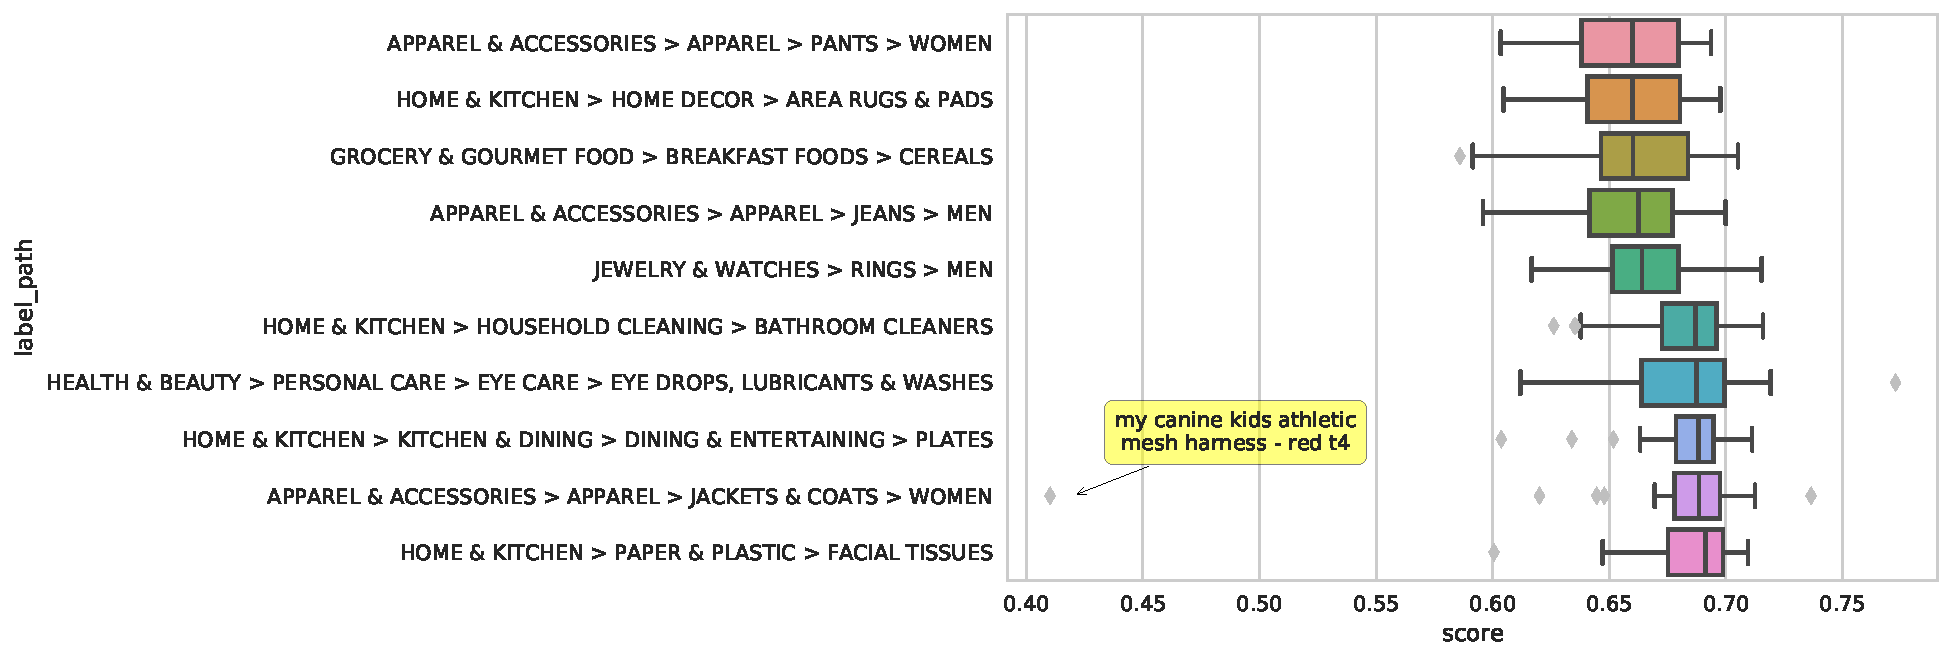
\includegraphics[width=\textwidth]{resources/noise-detect}
   \caption{Noisy training sample detection.  }
   \label{fig:noise-detect}
\end{subfigure}
\begin{subfigure}[b]{0.33\textwidth}
   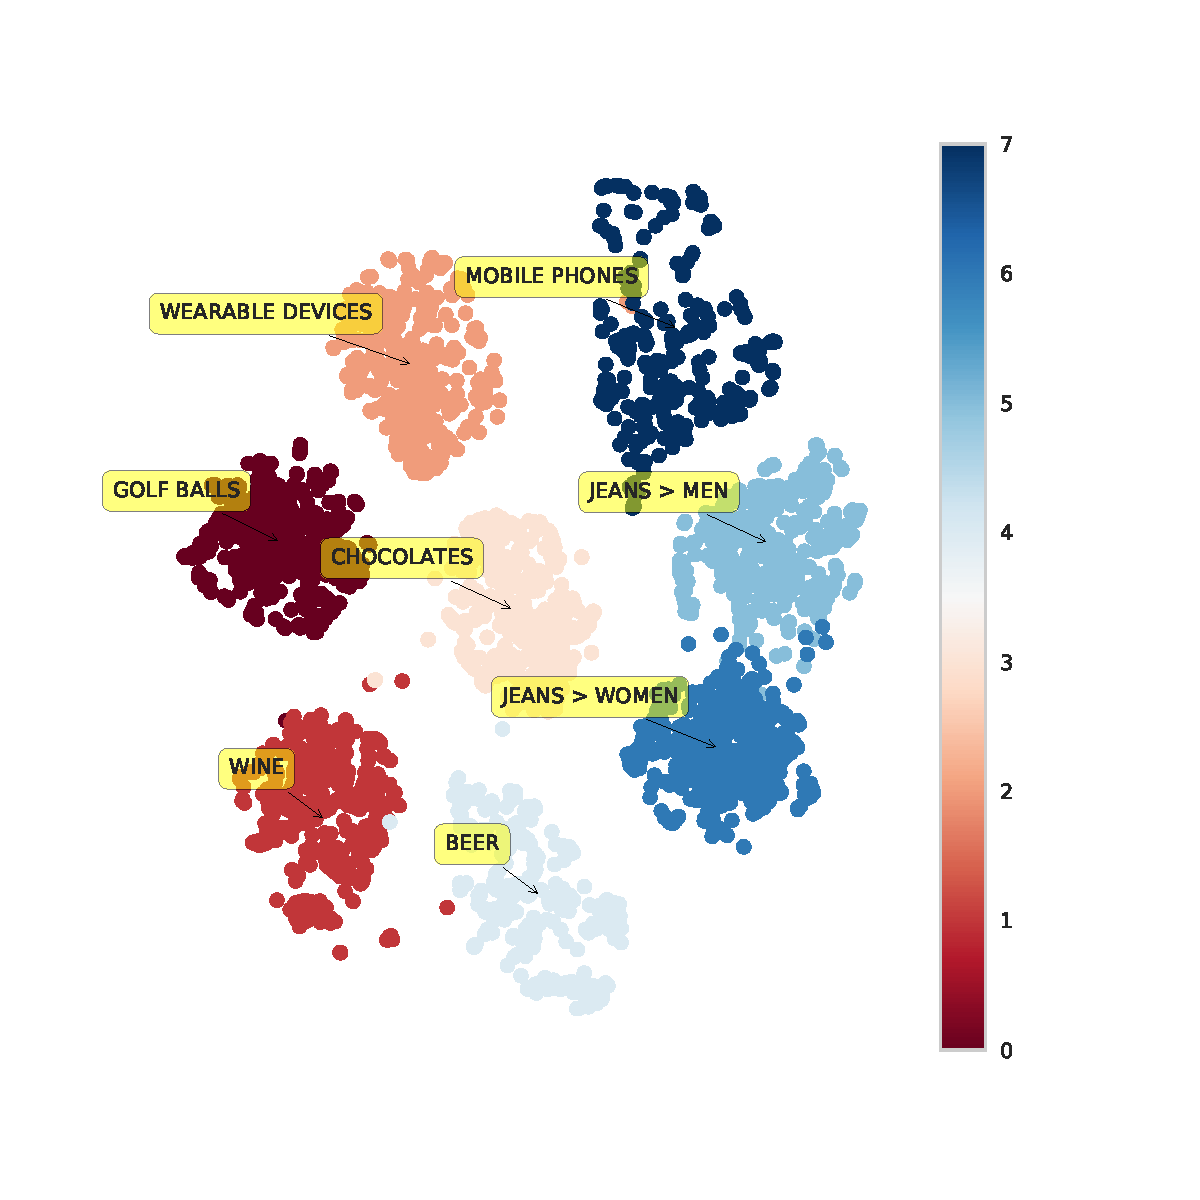
\includegraphics[width=\textwidth]{resources/cluster}
   \caption{Visualizations of item vector clusters.  }
   \label{fig:cluster}
\end{subfigure}
\begin{subfigure}[b]{0.3\textwidth}
   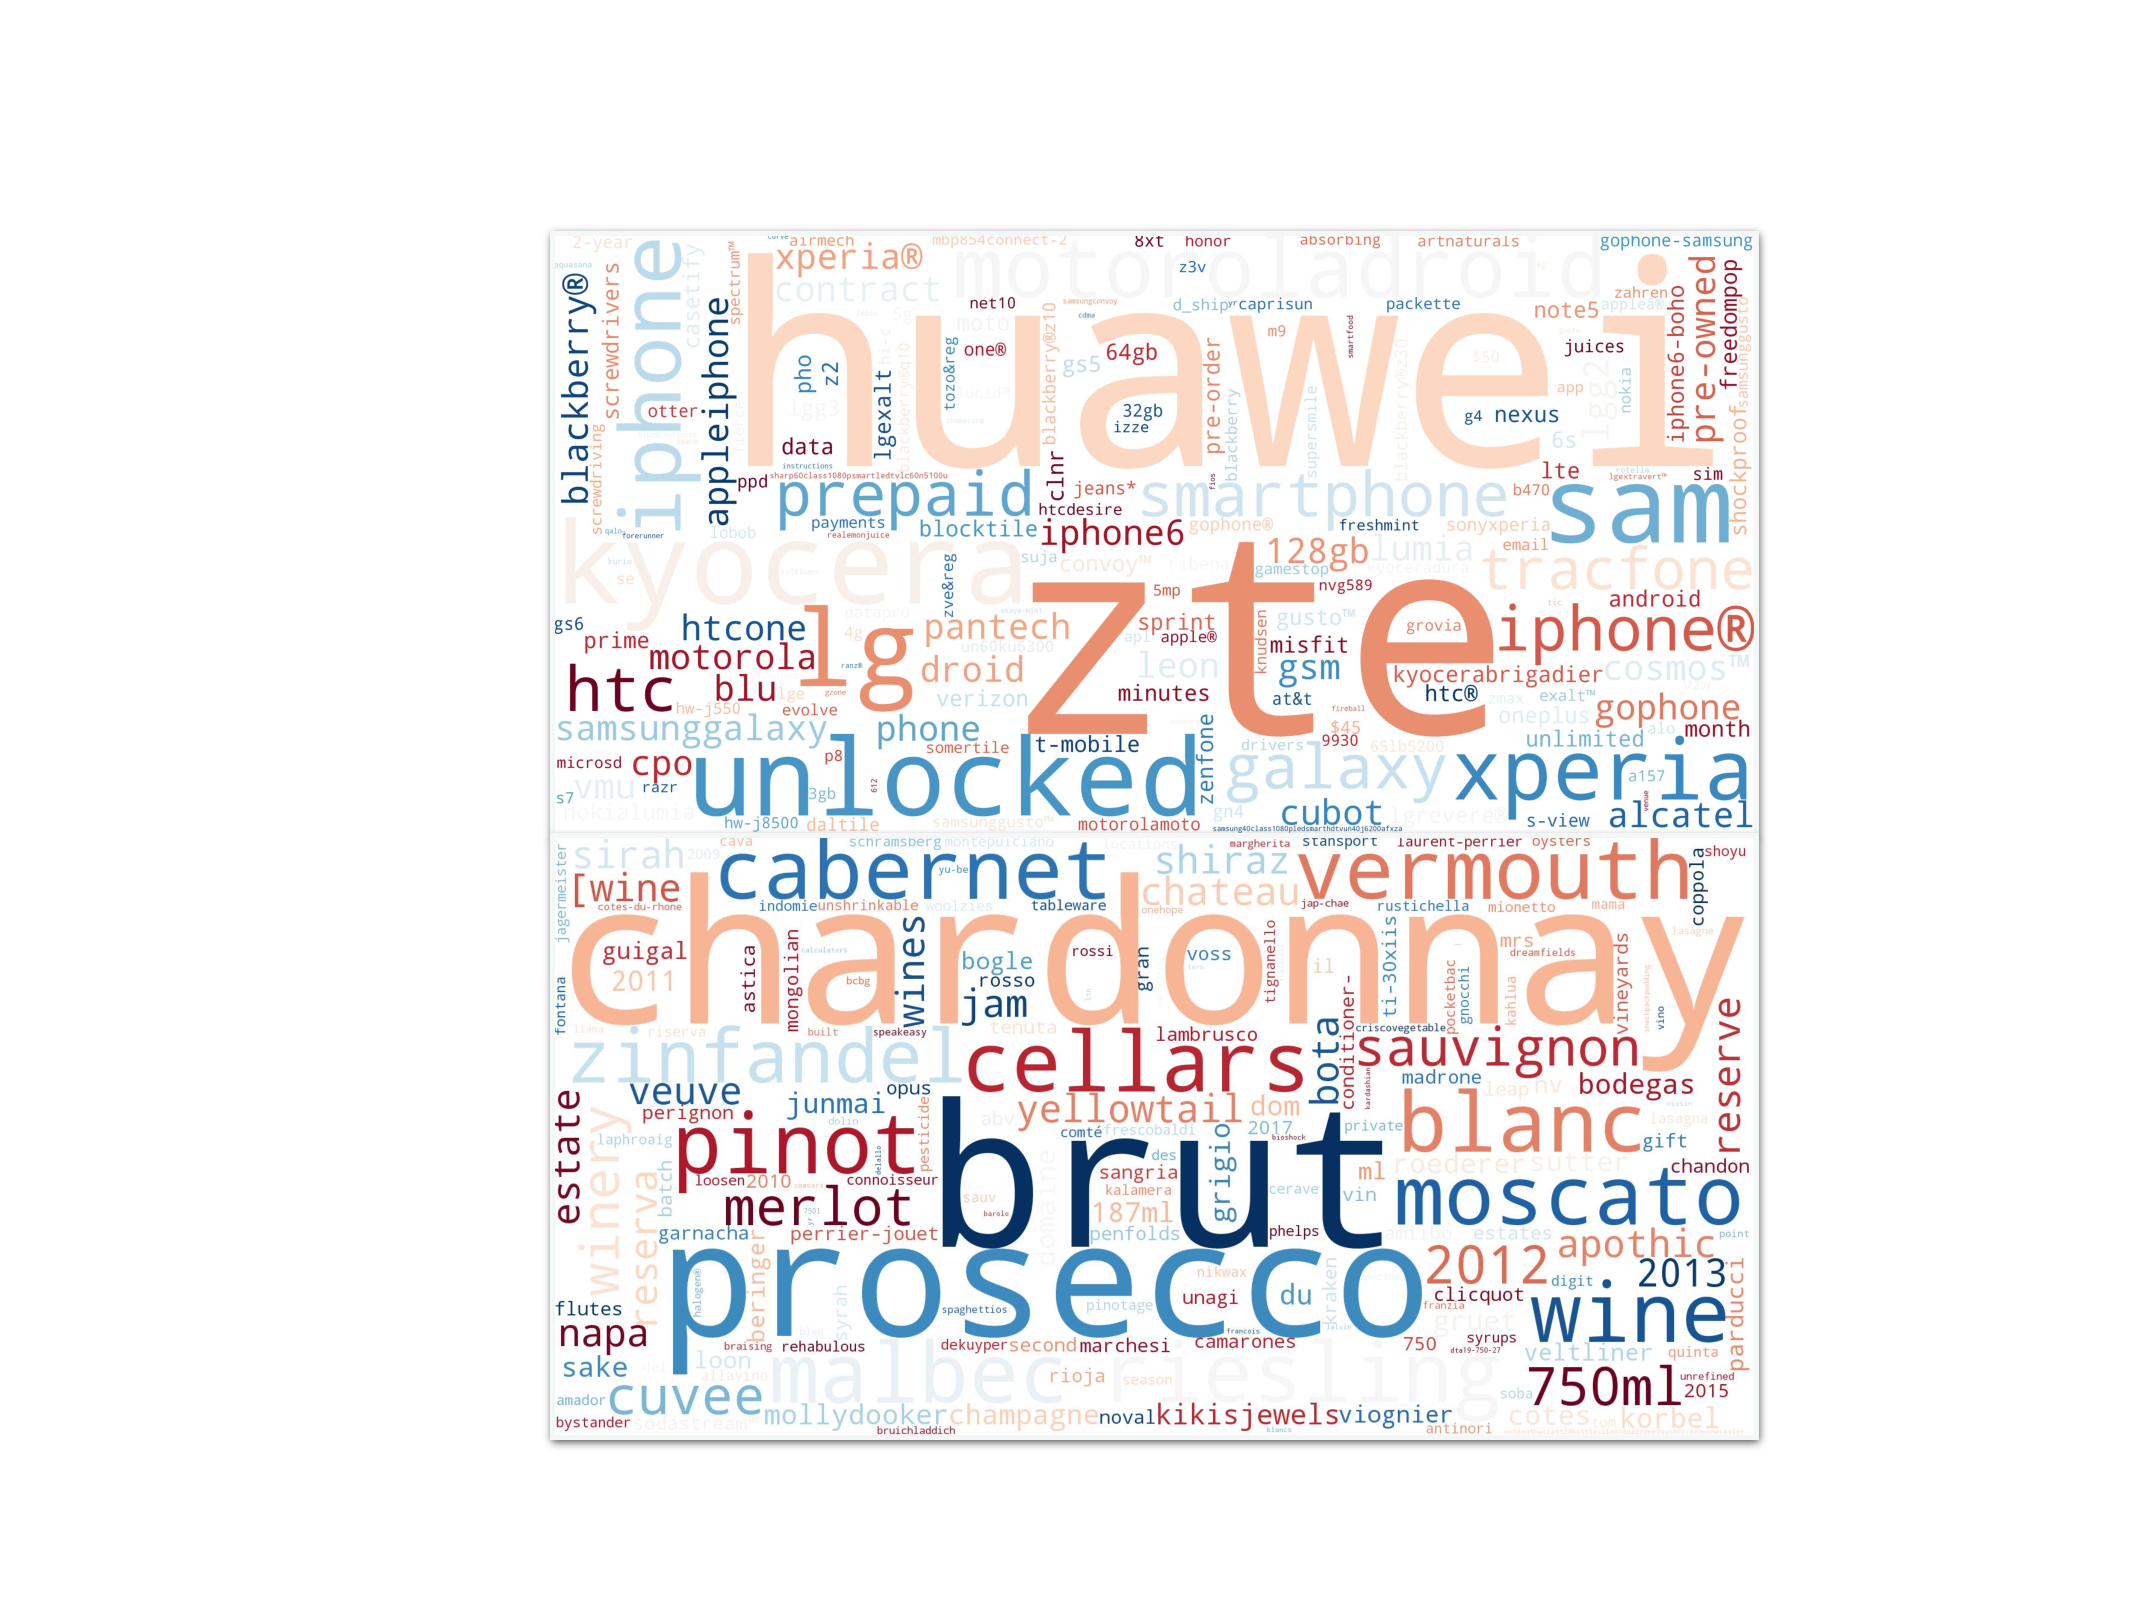
\includegraphics[width=\textwidth]{resources/wc}
   \caption{Top feature clouds.}
   \label{fig:wc}
\end{subfigure}
\caption{In (\ref{fig:noise-detect}) it shows eight categories and their training sample `confidence' scores distribution. Outliers are denoted by black dots. (\ref{fig:cluster}) visualizes the dense 50-dimensional item vectors that are projected onto the 2-dimensional space using t-SNE with 50 perplexity and PCA initialization. (\ref{fig:wc}) is generated from top key words in categories \emph{wine} (bottom) and \emph{mobile phones} (above).}
\end{figure*}

\subsection{De-noising Training Sample} % (fold)
\label{sub:de_noising_training_sample}

Items that are labeled incorrectly will affect the qualities of the categorization system if a lot of them are present in the dataset used for training. Noises get introduced into the training set either due to conflict or noisy business rules or because of the labeling process which is often labor-intensive and thus error-prone. Here we discuss an effective de-noising approach based on active learning \cite{culotta2005reducing}, which alternatively update the least `confident' items given the classifier or the classifier given the training data.


% subsection de_noising_training_sample (end)

\begin{table*}
  \caption{Strongest Unigram Features for Category Prediction}
  \label{tab:features}
  \begin{tabular}{cccccccl}
    \toprule
    JEANS > MEN	&	JEANS > WOMEN	&	WEARABLE DEVICES	&	 BEER	&	 WINE	&	CHOCOLATES	&	 GOLF BALLS	 & MOBILE PHONES \\
    \midrule
    brixton	&	jeans-	&	smartwatch	&	ipa	&	chardonnay	&	ferrero	&	titleist	&	zte	\\
    graduate	&	suki	&	misfit	&	ale	&	brut	&	m\&m	&	srixon	&	huawei	\\
    normandie	&	super-skinny	&	fitbit	&	beer	&	prosecco	&	lindt	&	callaway	&	kyocera	\\
    fit-	&	rips	&	jawbone	&	budweiser	&	riesling	&	hersheys	&	maxfli	&	unlocked	\\
    rude	&	wedgie	&	forerunner	&	lagunitas	&	pinot	&	m\&ms	&	volvik	&	sam	\\
    skinny-fit	&	straight-leg &	vivofit	&	heineken	&	malbec	&	milka	&	taylormade	&	lg	\\
    levi's\textregistered	&	pajamajeans	&	tracker	&	coors	&	cellars	&	snickers	&	pinnacle	&	xperia	\\
    501	&	stevie	&	fitness	&	lager	&	wine	&	kisses	&	bridgestone	&	iphone	\\
    a\&f	&	524\texttrademark	&	nike+	&	modelo	&	vermouth	&	kinder	&	balls	&	motoroladroid	\\
    527	&	524	&	pebble	&	shiner	&	moscato	&	cadbury	&	dozen	&	smartphone	\\
    sartor	&	5pkt	&	garmin	&	peroni	&	blanc	&	ghirardelli	&	distance	&	 iphone\textregistered	\\
    selvedge	&	jegg	&	withings	&	bottles	&	cabernet	&	brookside	&	wilson	&	galaxy	\\
    carpenter	&	rockstar	&	vivosmart	&	guinness	&	zinfandel	&	twix	&	golf	&	htc	\\
    stonewash	&	nouveau	&	activity	&	corona	&	sauvignon	&	butterfinger	&	cornmeal	&	prepaid	\\
    matchbox	&	seabreeze	&	smartband	&	sixpoint	&	750ml	&	godiva	&	flite	&	tracfone \\
    \bottomrule
  \end{tabular}
\end{table*}


